\chapter{Trial Results} 
\label{chap:trialResults}
%in this section i will first discuss the raw results of the trial, then discuss both the primary results (the raw data) and the secondary results (lessons on how the trial was run)

\section {Limitations of Trial}
The scope of the exploratory trial was limited after the Dissertation proposal due to timing of applicable grants. Some parts of the proposed design, including detection of PIPs, generation of targeted interventions, and wireless data delivery were reduced as a result, in scale in order to comply with the timing demands enforced by the supporting grants. The project was refocused on collecting physiologic and psychosocial data and post processing that data. The BKE was scrapped as a live updating entity, eliminating the requirement for a medical ontology.

The goal of the trial, was now to build and implement a system for data collection consisting of a non-intrusive sensor apparatus to collect psychometric data and a cellphone application to accumulate psychosocial data. The sensor would need to have its data manually downloaded each week by a visiting clinician. Detailed information about the sensor package can be found in \cref{chap:ProtoTypeBuildTest} : \nameref{chap:ProtoTypeBuildTest} .


\section{Exploratory Trial Initial Description}

Sethares et al. proposed a trial to assess the usefulness of the sensor design concepts including both the new sensor hardware and the cellphone application to collect somatic awareness data.  The trial was originally proposed to run from November 2013 through August 2014 \cite{KristenASethares2013}. Due to issues unrelated to research the first patient was not equipped with sensors until May 2014.

\begin{figure}
 \begin{center}
  \label{fig:CarePackage}
  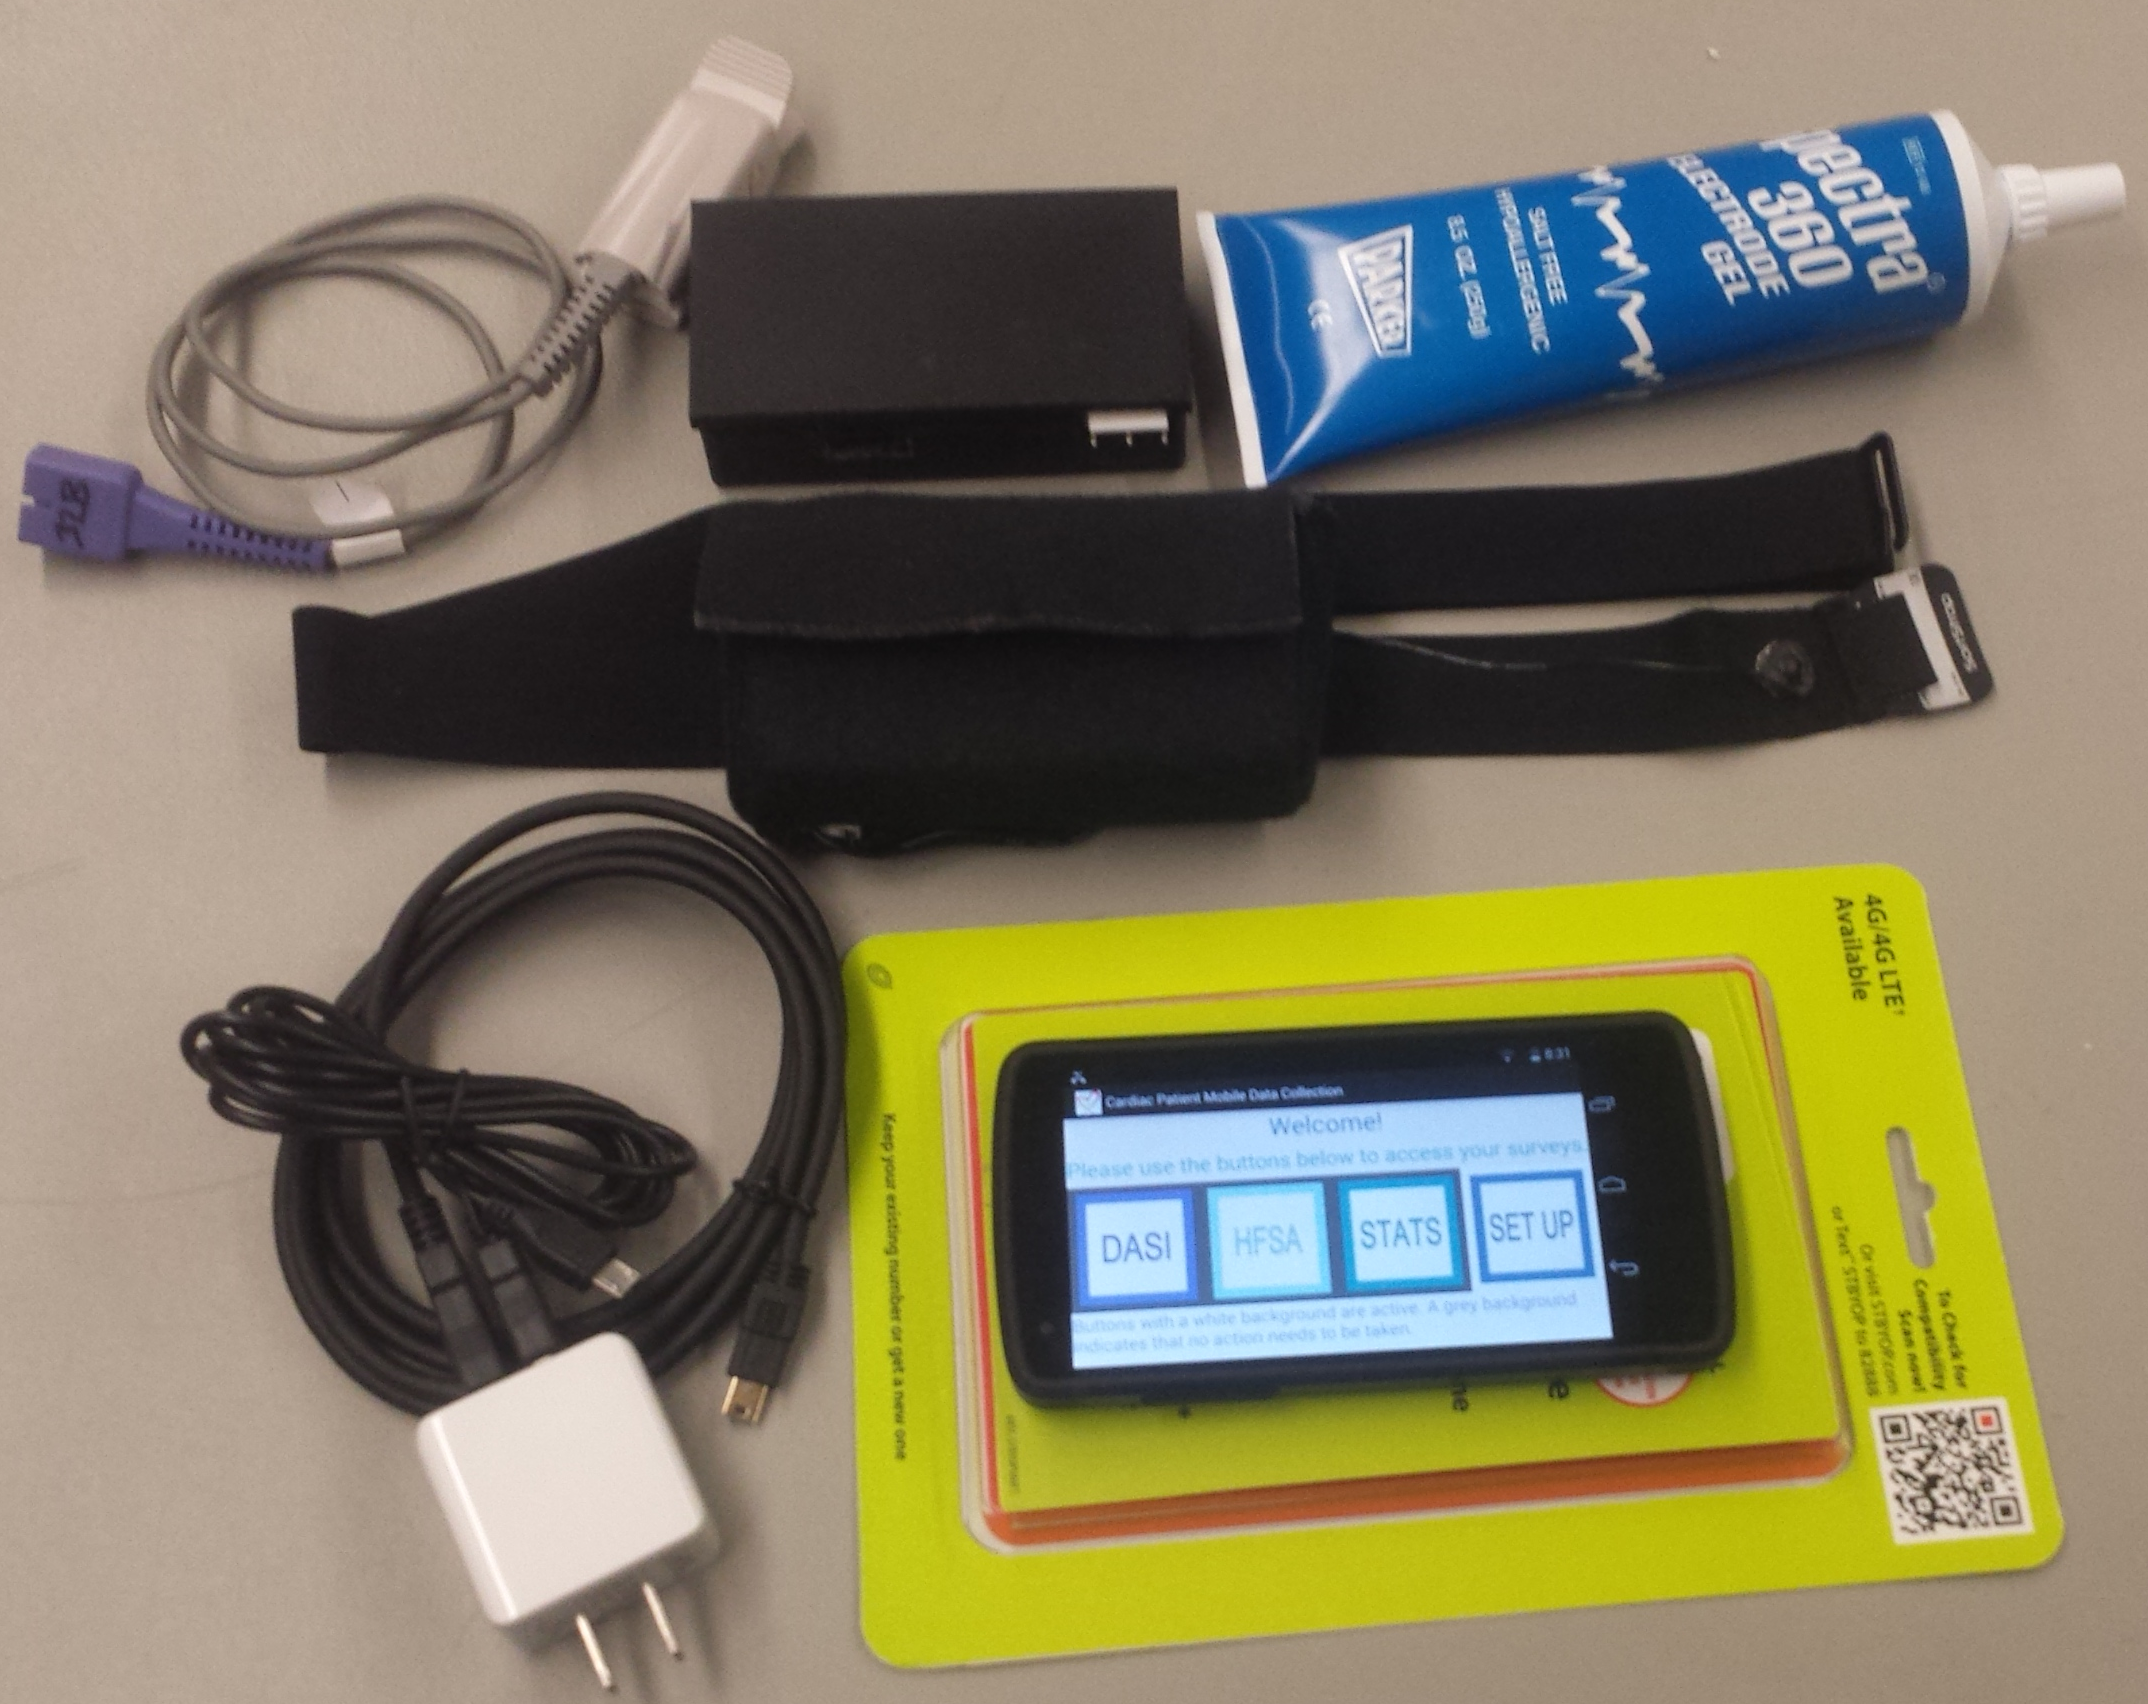
\includegraphics[scale=1,width=0.75\textwidth]{Images/carePackage.png} 
  \caption{Care package for each participant.} 
 \end{center}
\end{figure}



Each participant was provided with a package as shown in \cref{fig:CarePackage}:
\begin{itemize}
\item An lg nexus 5 cellphone with the heart monitor application
\item a sensor assembly
	\begin{itemize}
	\item a 3d printed enclosure
	\item a sensor board
	\item a modified polar(r) brand chest strap
	\item a fabric pouch
	\end{itemize}
\item a tube of electrode gel
\item a two port USB charger
\item a USB A to USB mini cable
\item a USB A to USB micro cable
\end{itemize}

The patient was instructed to wear the device during the day and to wear the finger clip, when convenient. The patient was instructed to take off the device and plug it in to charge at night . Additionally, the patient was given a smartphone, with a data plan, and shown how to use the survey application (app). 

\begin{figure}
 \begin{center}
  \label{fig:AndroidSplash}
  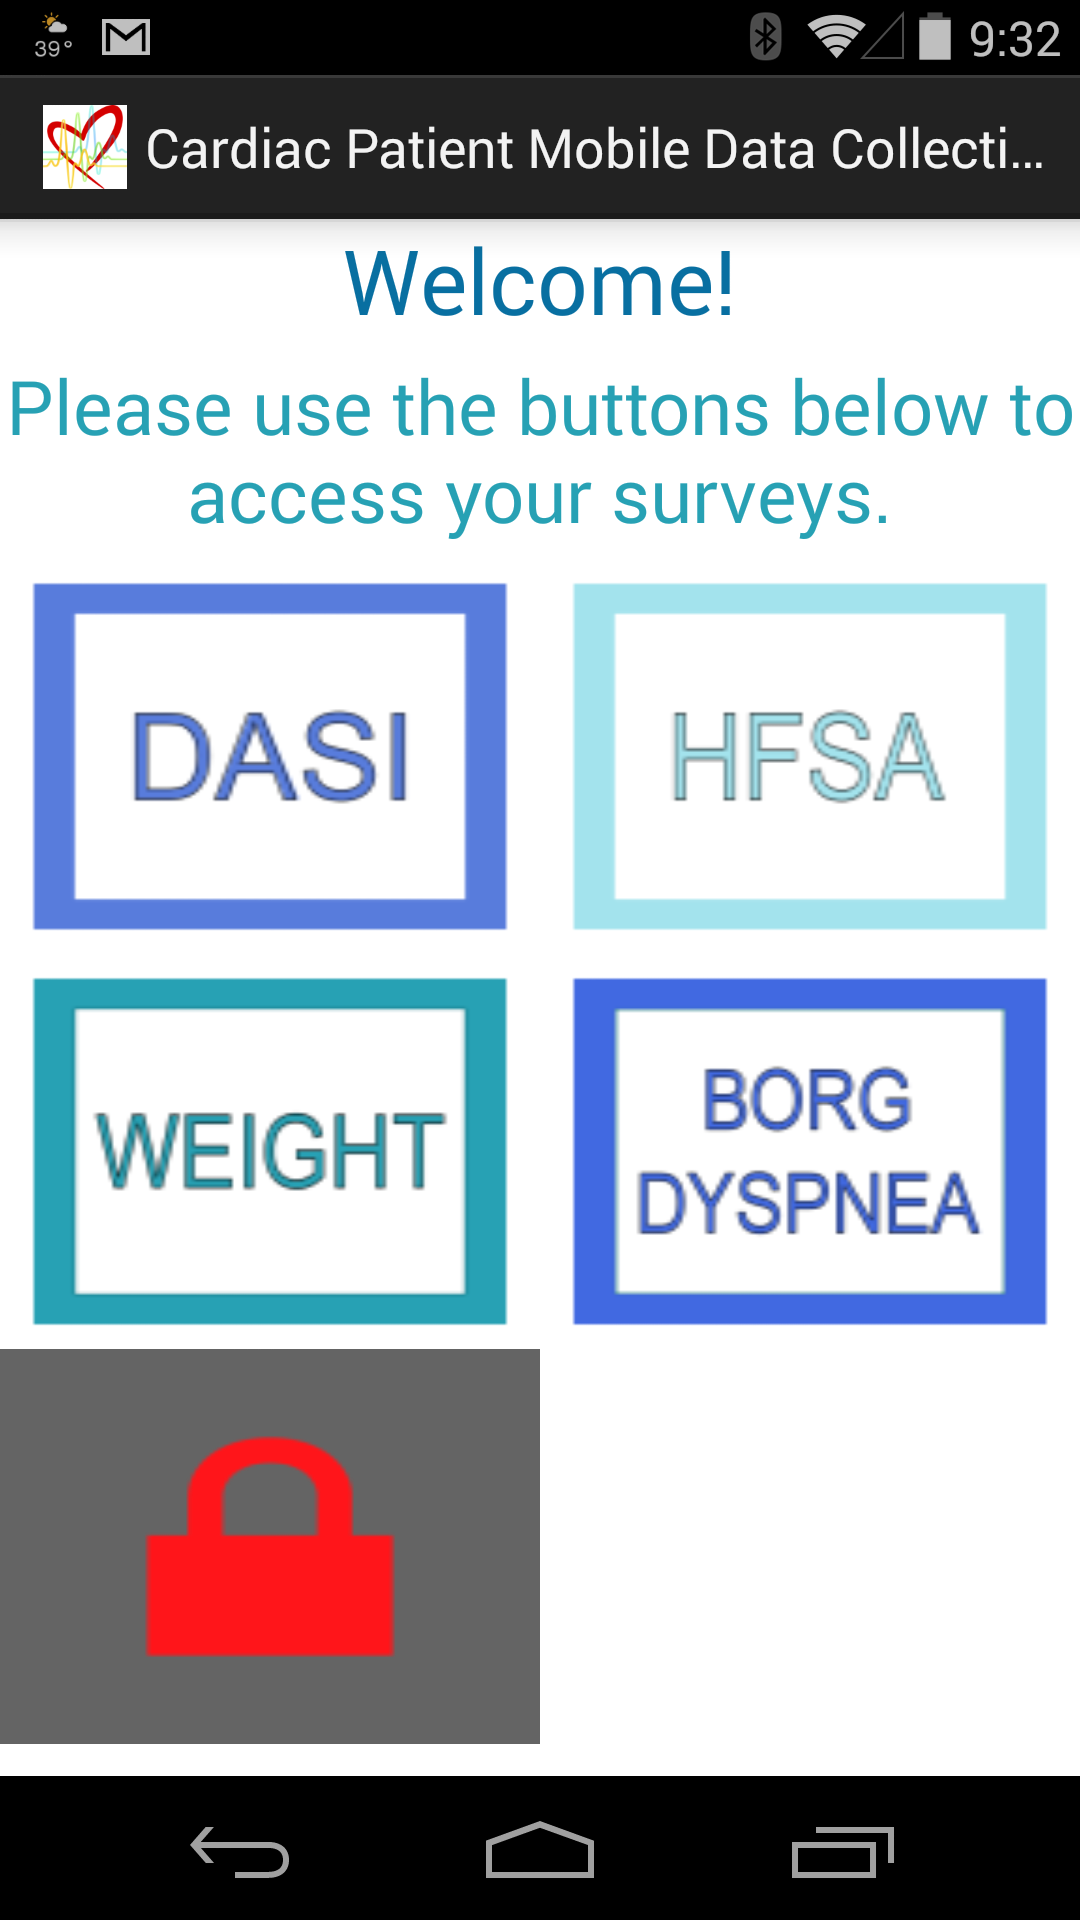
\includegraphics[scale=1,width=0.3\textwidth]{Images/AndroidSplash.png} 
  \caption{Main Screen for Smartphone Apps} 
 \end{center}
\end{figure}

\section{The Phone application}

The smartphone application was written in Java by an undergraduate researcher, based on previous masters projects in the MCHM research group \cite{Louro2013,Putin2011}. The application underwent several revisions over the course of the trial. \cref{fig:AndroidSplash} shows the initial screen presented to enrolled patients when they started the app. allowing for weight and dispnea data entry or to trigger a psychosocial survey.

The first iteration implemented a different version of one of the psychosocial assessment tools, using a 1-4 lickert scale, the instrument was supposed to have 0-5 with 0 indicating "I did not have that symptom". It also did not have the self reporting behaviors for COPD patient. Last, there was no alarm feature implemented inside the survey application to remind the patients to participate in the self care instruments.

\begin{figure}[ht]
\centering
  
  \begin{subfigure}[b]{0.3\textwidth}
  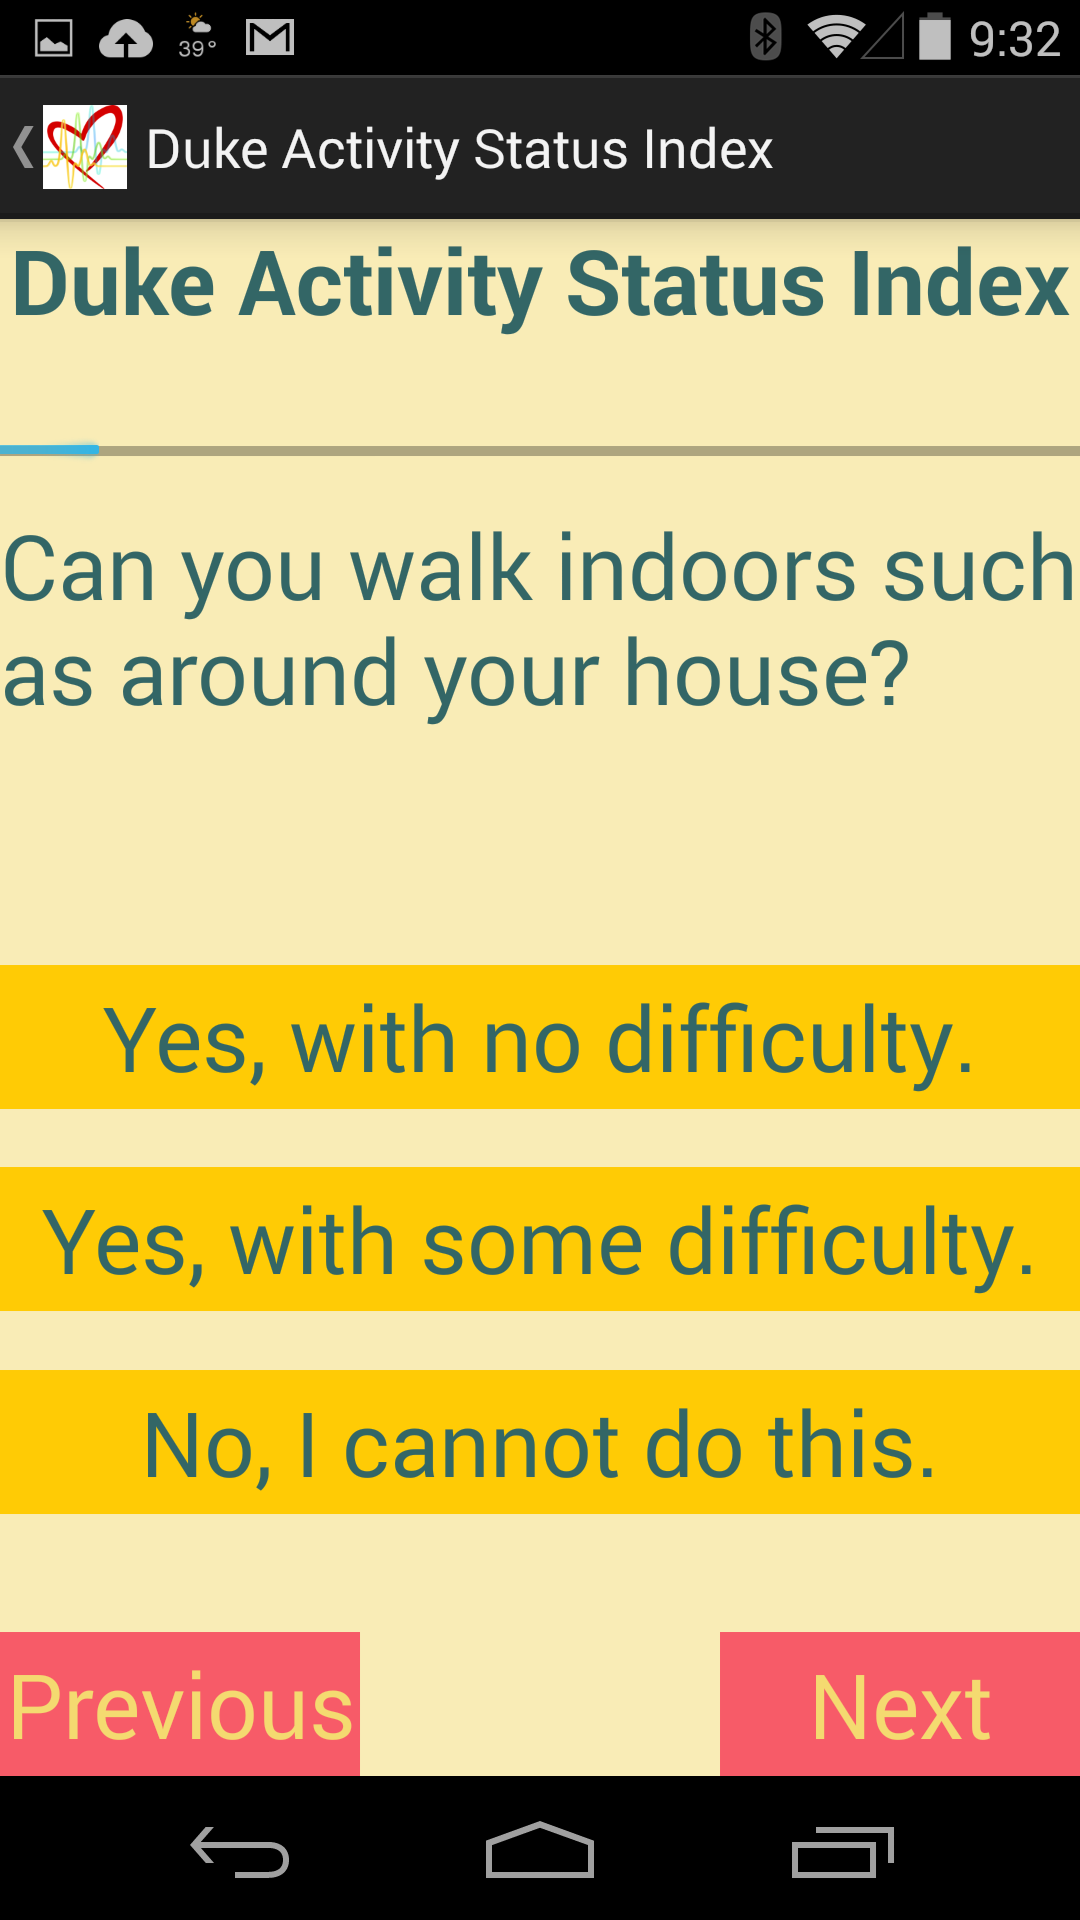
\includegraphics[scale=1,width=\textwidth]{Images/DASI.png}
  \caption{DASI Survey}
  \label{fig:DASI}
  \end{subfigure}
  ~
  \begin{subfigure}[b]{0.3\textwidth}
    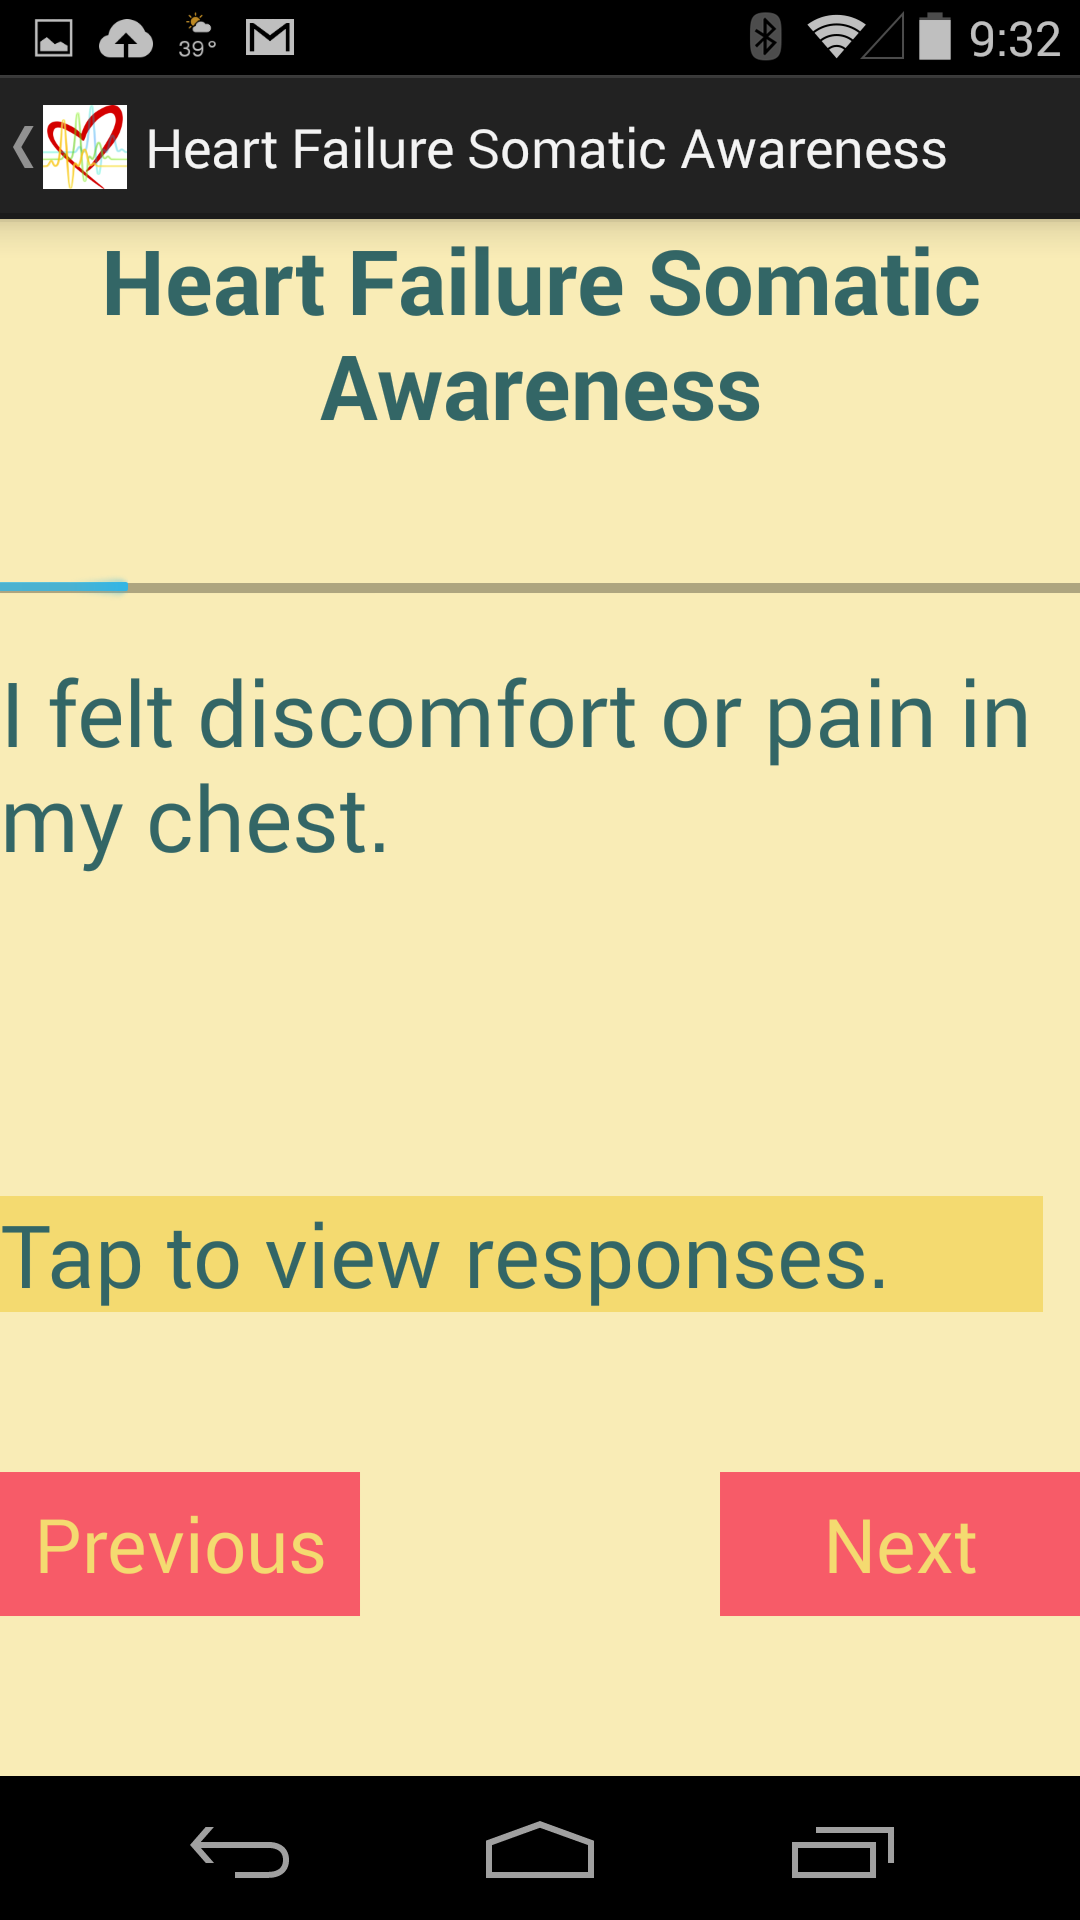
\includegraphics[scale=1,width=\textwidth]{Images/HFSA_question.png}
	\caption{HFSA Question}
  	\label{fig:HFSA_Q}
  \end{subfigure}
  ~
  \begin{subfigure}[b]{0.3\textwidth}
    	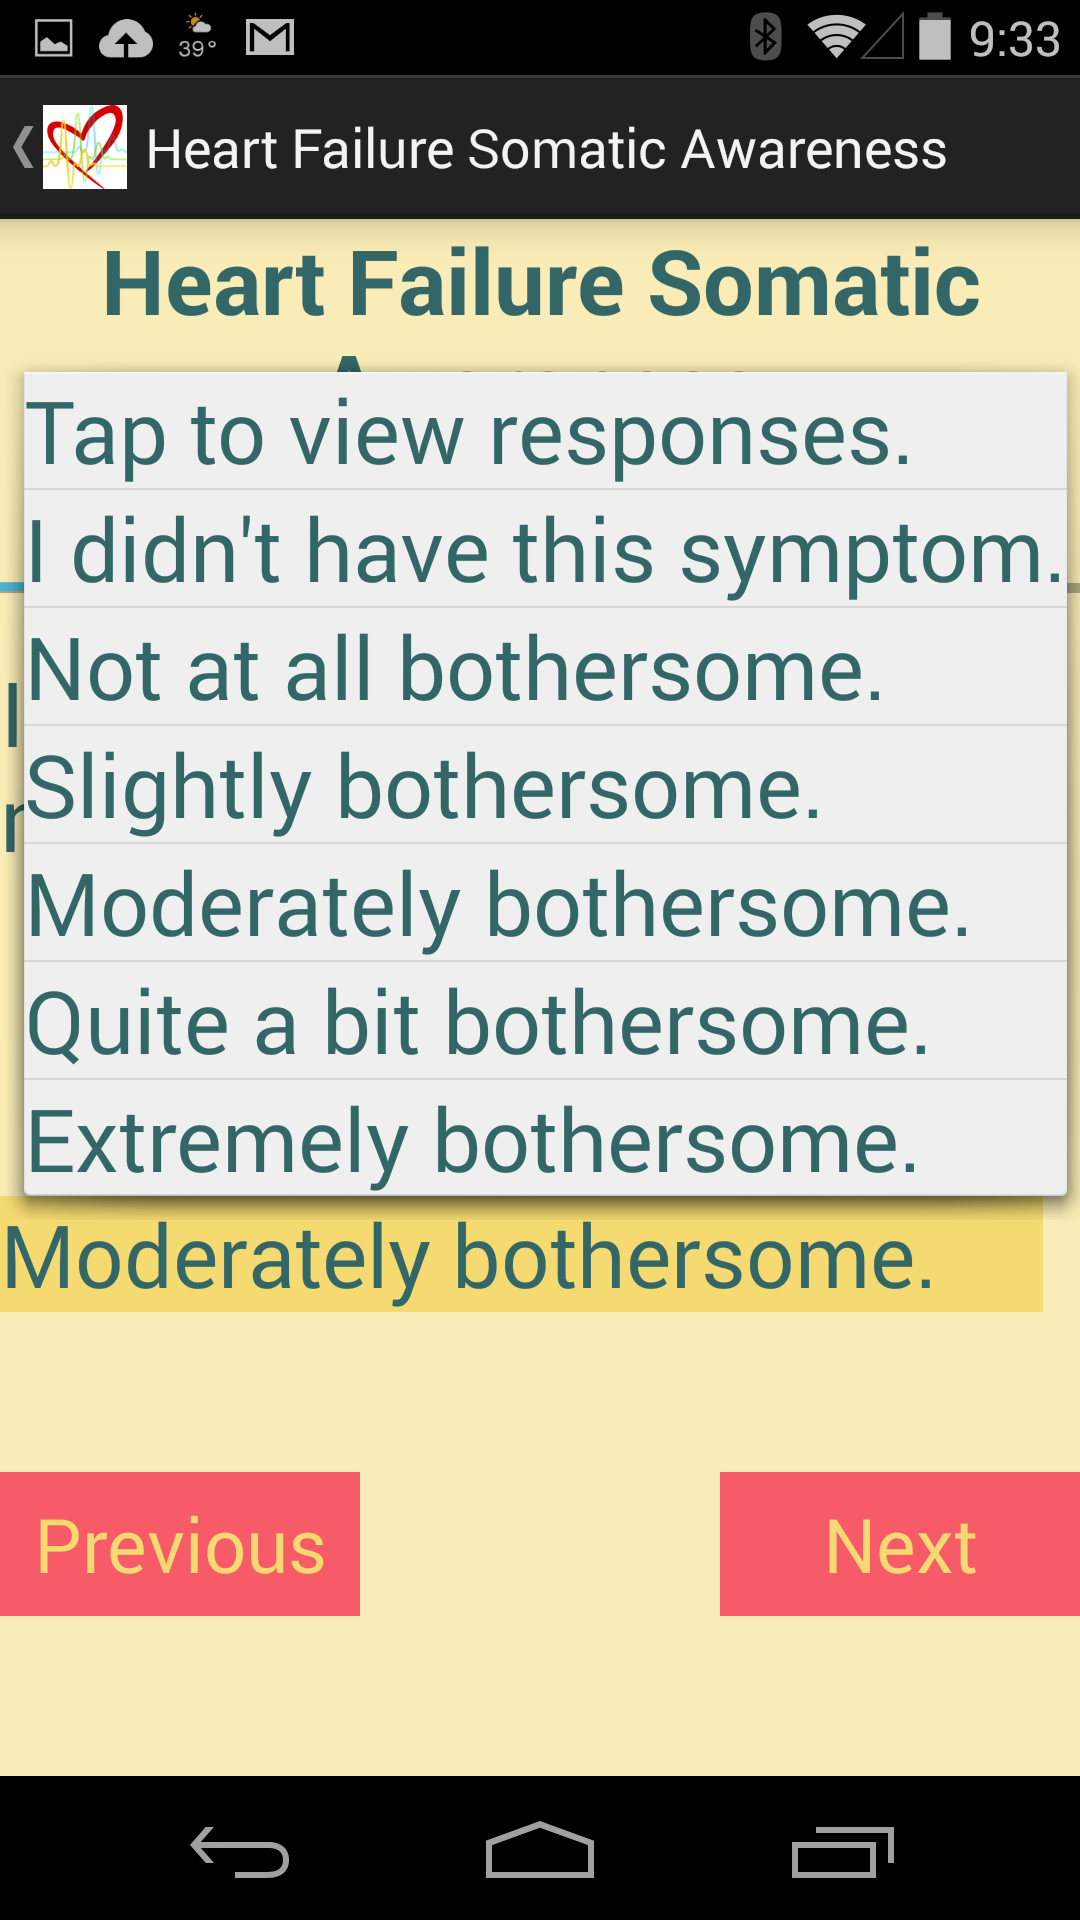
\includegraphics[scale=1,width=\textwidth]{Images/HFSA_answer.png}
  		\caption{HFSA Responses}
  		\label{fig:HFSA_R}
  \end{subfigure}
  \caption{Psychosocial Entry Screens} 
  \label{fig:AndroidSurveys}
\end{figure}

The timing of when the surveys should be administered was a reoccurring problem. Initially the phones clock alarm was used to remind the patients of when the surveys should be taken. This came to a sudden halt when one patient was unable to deactivate the alarm, only snooze it for 15 minutes at a time, for 3 days. The decision was made to remove the alarm feature from the protocol after this patient. Additionally, at the start of the trial, the patients were not allowed to take the survey instruments more than 3 times a week, as indicated by the initial proposal. However, the resulting user experience was suboptimal, the prevailing reaction to being unable to take a survey was the perception the patient had done something wrong, resulting in frustration. A modification was made to allow the surveys to be taken at any time.

Unfortunately, integrating the required fixes for the changed lickert scale introduced an error in the submission process for the HFSA instrument that went unnoticed for several months. It was ultimately fixed but the patient information was un recoverable.

Each survey was administered one question at a time, the different types of surveys each required a unique data entry technique as seen in \cref{fig:AndroidSurveys}. For the DASI, \cref{fig:DASI}, three buttons were available, pressing one, both chose the answer and advanced to the next question. For the HFSA, \cref{fig:HFSA_Q}, a dropdown box would be available to select an answer, \cref{fig:HFSA_R}, then the user would have to manually advance to the next question. 



\section{Trial Lessons learned}

\subsection{Lack of Time}
\paragraph{Back End Processing}
\paragraph{Testing}
\paragraph{Documentation}
\paragraph{Wearable Design}
\paragraph{Wireless update}
\paragraph{Live Results}
\paragraph{no alpha, straight to beta}


\subsection {Lost data}
\paragraph {too long between visits}
\paragraph {bad SDcard adapter}
\paragraph{excessive SD card handling}

\subsection{Lack of documentation}
\paragraph{cellphone user manual}
\paragraph{WHIP troubleshooting guide}
\paragraph{ digital surveys vs soft surveys}

\subsection{Communication Problems}

\subsubsection{patient - nurse communication}
\paragraph{cellphone usage}
\paragraph{proper strap placement/usage}

\subsubsection{Feature creep}
\paragraph{COPD - Borg Dispnea}
\paragraph{modified likert}
\paragraph{survey alarms}
\paragraph{strict survey -> anytime survey}

\subsubsection{nurse - engineer communication}
\paragraph{delay between problem observation and problem reporting}
\paragraph{no timely feedback on collected data}


\subsection{Loose protocol adherence}
\paragraph{ changes in survey protocol, database changes}
\paragraph{ changes in sensor useage (finger clip)}
\paragraph{ no calibration measurements}
\paragraph{ ECG Disconnected}
